% TEMPLATE for Usenix papers, specifically to meet requirements of
%  USENIX '05
% originally a template for producing IEEE-format articles using LaTeX.
%   written by Matthew Ward, CS Department, Worcester Polytechnic Institute.
% adapted by David Beazley for his excellent SWIG paper in Proceedings,
%   Tcl 96
% turned into a smartass generic template by De Clarke, with thanks to
%   both the above pioneers
% use at your own risk.  Complaints to /dev/null.
% make it two column with no page numbering, default is 10 point

% Munged by Fred Douglis <douglis@research.att.com> 10/97 to separate
% the .sty file from the LaTeX source template, so that people can
% more easily include the .sty file into an existing document.  Also
% changed to more closely follow the style guidelines as represented
% by the Word sample file. 

% Note that since 2010, USENIX does not require endnotes. If you want
% foot of page notes, don't include the endnotes package in the 
% usepackage command, below.

\documentclass[letterpaper,twocolumn,10pt]{article}
\usepackage{usenix,epsfig,endnotes}
\begin{document}

%don't want date printed
\date{}

%make title bold and 14 pt font (Latex default is non-bold, 16 pt)
\title{\Large \bf Robust Networks of Reputation for Client-Service Provider Interaction}

\author{
{\rm Miles Fertel}\\
\and
{\rm Abby Lyons}\\
\and
{\rm Emma Weil}\\
}

\maketitle

\thispagestyle{empty}


\section*{Abstract}
\textbf{In the age of the Internet, it is difficult for a service provider (SP) to determine whether their potential online clients on some online marketplace are trustworthy, or vice versa. This is particularly challenging when users do not want their legal identities known by members of the community, but would like a sense of accountability and reputation tracking while performing transactions. PGP Web of Trust offers a basis for a network of trust, but the structure benefits the creation of make fake accounts. To address this, we propose a centralized system for keeping track of users and reputations in order to create a network of trust between users. Additionally, unlike other proposed systems, we do not need to keep track of individual transactions in order to prevent re-rating. Our system, \textit{Silkworm}\endnote{Silkworms spin cocoons of thread that are both protective and complex.}, works on top of existing communication/marketplace environments and allows for pseudonymous users to rate the quality of their transactions with other pseudonymous users. The impact of the rating on reputation score is determined by each rater's reputation, which improves the reliability of user reputations.}

\section{Introduction}
PGP, or Pretty Good Privacy, is one of the earliest encryption tools designed for public use. Its use cases are not quite the same as the one our system is designed for, but it is the backbone of many related systems, like the PGP Web of Trust. PGP relies on each user having a public key certificate, which includes an owner ID, key ID, and the public key itself; the key ID is then used as their primary identifier instead of their real name. Trust in PGP is defined as confidence in the binding between the key ID and the public key~\cite{PGPWebTrust}. While we have the same notion of trust--that a Silkworm channel ID actually belongs to a user who claims that it is theirs--we focus primarily on a different standard, reputation, which we define as confidence that a person in the marketplace has history of being responsible with regards to their transactions.

The PGP Web of Trust is a system designed for propagating trust for key-identity pairing certificates through \textit{introducers}. This is necessary to do because of there is no central authority on public key identities. Introducers allow person $A$, who directly trusts person $B$, to trust person $C$, who has a certificate signed by $B$. A fault in this system is that one can manipulate their own trust rating by creating many false users to sign one's certificate. In our system, this is not possible because a rating can only be given after a valid (mutually agreed upon) transaction, and because reputation can only be increased once per set of users.

Since the introduction of the PGP Web of Trust, a few important modifications have been made~\cite{ImprovingPGPWebTrust}. One is the expansion of the score space in the Web of Trust to range between \{-1,1\} instead of \{0,1\}, where a score of -1 indicates that a feedback provider thinks a public key certificate is \textit{not} authentic. This allows certificates to have a negative trust rating if many users feel it is not trustworthy, instead of maintaining a trust score of 0, which is the same as the score of a new or unknown certificate. We incorporate the expanded range to indicate a negative reputation, in contrast to a new user's reputation which would have a score of 0.

We improve upon the Web of Trust's reputation architecture by constructing the notion of \textit{trust transactions}. A trust transaction is a two way interaction between users in the system in which the reputation of each user is updated based on a given rating. This translates to a Web of Trust style reputation score increment, but scaled by the reporting user's reputation. This allow us propagate reputation with greater accuracy than PGP Web of Trust. We also realize that a community will have varying levels of trust in their SPs, so we allow for varying base reputation values given a user's role. This amounts to a standalone reputation verification system that is more accurate, generalizable, and accessible than the PGP Web of Trust.

\section{Background and Motivation}

There are already many trust and/or reputation systems in place for specific services, like Uber and AirBnB. However, these are specific to their respective applications and cannot easily be used outside their contexts. Additionally, these systems include many identifying pieces of information, like license plate, name, address, and potentially even a photograph of the user. Given that these models are unfeasible in marketplaces where users care about protecting their identity, it is important to have some notion of reputation for each type of user. This is especially the case if the SPs work freelance or if either party might be in danger given the nature of the work. There are also systems, like PGP's Web of Trust, and even other anonymous reputation networks, that depend on the ability to keep track of transactions or signing of certificates in order to later revoke them. We believe it is valuable to destroy transactions after they have happened, such that an attacker cannot reassemble graphs of transactions between users in order to infer identities.  

In our design, we take a somewhat contentious approach by acknowledging that the system will likely be used by people who may be committing illegal activities. However, we hope to allow people working in dangerous markets to have a stronger sense of safety when working with others. For example, many services that make transactions between people easier and safer explicitly disallow transactions from including sex work. Motivation for these types of decisions is in part because it is generally hard to tell who is trustworthy online if they are not part of an established marketplace with a rating system, and is, in this example, made more difficult because the image of the sex worker has been exploited in online scams to lure foolish victims.\endnote{Like our idiot friend Todd.} We design this system so that someone can effectively refuse to do business with another person if they are not using Silkworm to keep track of their accountability or if their reputation score is questionable. This gives both the client and SP the power to make safer purchases. 

\section{Architecture}
A user will access the Silkworm application (web, mobile, etc). We assume in this case that the user has a secure and private internet connection.
Silkworm is then structured into user-generated \textit{channels} that represent some community. For instance, a channel might represent users who sell furniture on Craigslist, or users on a dating site used by sex workers. A user could potentially create multiple Silkworm accounts to become a user on a channel multiple times, but as we will show, there is no benefit to having multiple accounts.

\subsection{Channel Structure}
We provide a distinction between \textit{public} channels, in which there are no restrictions on who can join, and \textit{private} channels, in which one can only join if a current member invites them. Private channels are especially useful for the special case of an existing community migrating to Silkworm, in which we can assume that many users know each other by some degree of separation. Private channels have stronger guarantees of a true reputation score, because we can assume that more users are genuine and trustworthy due to them being vetted by others and allowed in the channel. We will go more in depth on the distinction in Section 4.

Public channels are visible from the main interface of Silkworm, such that anyone can join them by creating an account with that channel. A user who join's a public channel without being invited will be assigned a base reputation score $\beta$. All accounts are managed centrally, but accounts on different channels are have no centralized link, which is important for the case of a user's account on one channel being infiltrated, as an attacked cannot use that knowledge to infiltrate the user's account on another channel. Private channels are not visible from the main interface, and instead, one must have both an ID for the channel itself and also a single-use code that will be generated by the user who is inviting the new user. Every channel will have a counter of how many users are in the community at that time, such that a new user can gauge how well-used the channel is. Neither type of channel will list the IDs of users in the channel, such that one cannot have arbitrary access to lists of IDs. We will address channel creation more in section $3.3$. 

\subsection{User Account Structure}

Each user on a channel will log into it with a username and password, which we can assume will be strong enough such that they are not at risk of having their username and password guessed. A third piece of information is generated per user in a channel, called a Silkworm ID. This ID will be how user's identify themselves in a channel. This allows users to maintain easier-to-remember usernames for logging into their accounts, but a unique identifier for use in transactions that will have no relation to the user's general online identity. This is important because it is possible to try to use someone's public-facing pseudonym to track their other online accounts (if they use the same username for multiple services), but it is annoying for users to remember an arbitrary ID. A user can view their own ID while logged into a specific channel. As an extra measure against attackers, logins will be rate-limited, and trying to log in will take a constant amount of time, such that one could not use a timing attack to see if a certain username is part of a channel. Additionally, transactions will take a constant amount of time, such that one could not see based on server response time if an ID is valid or not when a transaction is sent. More on Transactions will be in Section $3.4$. 
The following information is associated with an account on a channel: username, password, Silkworm ID, reputation score, number of completed transactions, incomplete transaction flag (ITF), a list of invited user structures. This structure is expanded upon more in the next section. Of those, only Silkworm ID, reputation score, number of completed transactions, and ITF are visible to another user in the channel. The number of transactions is important to give context for a neutral-seeming reputation score, which will tell a user if another user more likely to just be a new user or to be a malicious user with some number of negative transactions. The ITF is important for making sure a user cannot leverage refusal to complete a transaction in the case they know the rating they will receive will be negative. The public interface of Silkworm uses the reputation score of a given user to calculate a human readable rating based on the percentile a reputation score falls into relative to the community. Again, this system is better at proving that someone is reputable than that they are malicious, although we have protections against the latter. 

\subsection{Invitation Scheme and Channel Creation}

\subsubsection{Invitations}
Within a given channel, whether private or public, it is sensible for users to be able to invite other users to the channel. We provide the functionality for invitations to act as references. On invitation, an inviting member of a channel can select a level of trustworthiness of an invitee. Given the selected level, the new user's base reputation score will be a function of the inviting user's reputation according to the algorithm in $3.4.2$. The key insight is that when a user selects a trust level above "No trust", the reputations of the two user's are linked. If a user were to invite someone who became known as malicious, after endowing them with reputation, the inviter's reputation would decrease. As well, a user with low reputation can invite a new user to a community, but the new user will maximally have the inviting user's reputation score ($r$) if $r$ is below $\beta$. Additionally, we only allow users to generate an invitation code to a private channel if are the creator of the channel or if they have increased their own reputation by some amount, where some net unit of increase can earn a user an invitation. This helps prevent the case in which a malicious user is able to enter a private channel with some relatively good base reputation and then invite some other number of malicious users who inherit the same base reputation, as the original malicious users will not be able to invite more malicious users without putting time into increasing their own reputation by some amount. 

\subsubsection{Channel Creation}
Any user can create a channel, and we may consider some type of stricter moderation if there are many duplicate channels being created for the same thing. Generally, however, we can assume that a user will join whichever channel has the most members for a given type of community. Public communities will be sorted by area and type of transaction in order to make it easier to find the correct one, ex. a channel for Craigslist purchasers/sellers of goods in Boston. Channels that are public will have the number of members, total reputation score of all members and total number of transactions of all members as visible information before joining, such that one can avoid well-populated but unused channels or channels that sparsely populated. Additionally, one can only complete a transaction with a user inside of an agreed upon channel, so a user can decide to not do business with another if they deem the suggest channel to be suspicious.  

The creator of a channel, along with all users added to a channel during its creation, will have some base level of reputation assigned to them, such that new users to the channel can actually accumulate reputation. In order to avoid maliciously generated channels in which many users are created in it that all rate each other, including the creator (such that there is actually some non-base-level reputation score being taken into account when propagating it), we can flag channels in which there are frequent incomplete transactions. We can also have commonly used channels be endorsed by the service they complement, i.e. Craigslist itself has a link to its "official" Silkworm channel, and all others should be assumed invalid. These are not a perfect solutions, but most networks of trust/reputation do not do that well in scenarios with a collusion of malicious users \cite{ImprovingPGPWebTrust}, and we will expand on this topic in section 5.2 Known Challenges. 
%

\subsection{Transactions}
In a typical use case, two users on a communication platform would be able to view or send each other their Silkworm IDs and agree on an amount of time to give each other before expecting the transaction to be complete. To initialize a transaction through Silkworm between users $A$ and $B$ on the same channel:
\begin{enumerate}
    \item User $A$ logs into their Silkworm account on the appropriate channel for the communication platform, and searches for the ID of user $B$. At this point, $A$ can see $B$'s reputation score and can choose whether to start a transaction.
    \item $B$ must also log into their Silkworm account on the channel, and type in the ID of $A$, at which point they can also see $A$'s score. Until $B$ also chooses to start a transaction with $A$, $B$ does not know that $A$ has attempted to start a transaction with them.
    \item Once both users have notified Silkworm that they would like to start a transaction with the other's ID with the same time value, they are notified that the transaction has started.
\end{enumerate} 
Initializing a transaction also functions as a handshake, because it verifies that the two users on the communication platforms are in fact the respective owners of those Silkworm IDs by nature of recognizing the initiated transaction. Users only see that others have started a transaction with them when they actively initiate the other end of it, such that we do not have to worry about a case in which a malicious user gives out an ID to an account they do not own. Any pending uninitialized transactions (where $A$ has indicated to Silkworm that they would like to work with $B$, but $B$ has not indicated that they would like to work with $A$) will expire and be discarded after some amount of time (24 hours). Additionally, transactions cannot be reinitialized while they are still pending, unless the user revokes their pending transaction. Request revocation cannot happen after the transaction has been initialized, but in cases where both parties mutually decide that they no longer wish to perform the transaction, they can simply leave each other neutral ratings.  

To complete a transaction, $A$ and $B$ must submit ratings of -1 (negative experience), 0 (neutral experience in which one does not necessarily want to attest to the reputability of the other user), or 1 (positive experience) for each other. After both have submitted a score, the transaction and its ratings will be closed and used for the reputation update, and then securely deleted from the system, and only at this point will both users be able to see their updated reputation scores. If the transaction does not get closed within the amount of time agreed on (for instance, because one of the parties was malicious and does not want to let the negative rating affect them, or because a person was harmed and cannot respond from their account), a flag will be attached to the account of the user who has not submitted a rating to alert other users in the channel that they are the reason for an unfinished transaction.


%   Algorithm / reputation propagation 
\subsection{Algorithm of Reputation Propagation}
A user's reputation score is a function of their transaction score $t$ and their references (e.g. invites). The formula for a user's total reputation, $r$, is described in $3.5.2$.
\subsubsection{Transactions}
After a transaction has closed, and each user has submitted a rating of the other, we update the transaction reputation of each within the channel by the following formula:
\[t_{new} = t_{old} + \mu \left( rating \times \frac{r_{parter}}{\sum r_{community}}\right)\]
Simply stated, we generate a user's post-transaction reputation by incrementing their old reputation by the transaction partner's rating of the interaction, scaled by a heuristic of the partner's percentage share of the total reputation score of the community. This requires that Silkworm maintains the total reputation as part of the channel metadata. $\mu$ is a mobility constant defined by the implementation of Silkworm such that it is possible to scale how easy it is to go up or down in reputation. This can be exposed to channels, or defined globally. We address the selection of this constant more in section $5.2$.

\subsubsection{Invitations}
The Silkworm application internally manages a list of the users each user has invited to a given channel in the form of user structures. Each structure in the list contains:
\begin{itemize}
    \item The Silkworm ID of the invited user
    \item The base reputation level of the invited user
    \item The trust rating, $\tau$, of the invited user
\end{itemize}

An invite results in the base reputation of a new user according to:
\[r_{invitee} = min(\beta + \frac{\tau}{\gamma} r_{inviter}, r_{inviter})\]
Where:
\begin{itemize}
    \item $\beta$ is the base reputation of a of an uninvited user in a public channel.
    \item $\tau$ is a value generated from the trustworthiness rating provided by the inviter.
    \item $\gamma$ is the endowment constant, a scaling value representing how much of an inviter's reputation can be endowed to the invited user.
\end{itemize}
When an inviter provides a trust rating resulting in a non-zero $\tau$, their reputation score then becomes linked to the invited user such that their reputation is calculable by:
\[ r_{inviter} = t_{inviter} + \sum_{i = 0}^{invitees} \frac{\tau}{\rho}(r_{i} - r_{base}) \]
Where $\rho$ is a backflow constant representing how much an invitee's change in reputation should impact the inviter's reputation. This, as well, considers how trustworthy the new user was rated to be.  This formula is computed in order to generate a user's reputation score during the handshake phase of a transaction.

\section{Use Cases and Walk Through}
In this section we will fully describe a use case and vision for both a public and private channel.

\subsection{Public Channel Case}
An example of a community channel that may exist publicly on Silkworm is a group of people who buy and sell goods on Craigslist in Boston. In this scenario, a seller on Craigslist will list their item on the website in the regular format. The seller has a Silkworm account on the Craigslist:Boston:Goods channel. A person who is interested in the item will initiate communication as usual with the seller through the seller's email address. Either the seller or buyer will initially mention Silkworm within the terms of agreement to starting the purchase. If either party does not have Silkworm, the other user will suggest they create an account in the Craigslist:Boston:Goods channel. If they refuse, the seller or buyer can refuse to do service with them. 

If/when both parties are on Silkworm, each will look up the other's ID and confirm that eachother's reputation score is high enough given the risk involved with the transaction (a client may not care if the person with the goods is super trustworthy if the items are free or very inexpensive, but would care much more if the item were costly). The users would then agree on an amount of time to wait before the transaction should be complete and enter that into Silkworm, such that they can have a few days of leeway if the item will not actually be exchanged for some number of days. Then they send each other's IDs a transaction request with the time window, and when the requests match up in both subjects and time window, the transaction will be officially opened.

Once the transaction is opened, the only way to close it is by having both users rate each other. If something happens where one user backs out before the item is technically exchanged, good communication skills about the situation can still leave an honest buyer/seller with an unchanged reputation (where the other party gives them a neutral rating). If the transaction is completed as expected, the users will rate each other positively, and the user's reputations will update based on our propagation algorithm, and each user's total number of completed transactions will be incremented. If a transaction is never fully completed, because one or both parties never rate the interaction, then whoever did not rate the interaction within the time frame of the transaction will have a flag visible next to their ID's reputation score, which will warn other users that this person has something to hide. 

\subsection{Private Channel Case}
A an example of a community channel that may exist privately on Silkworm is a group of online sex workers who primarily use pseudonymous dating and messaging websites in order to find and interact with potential clients. In this case, the basic usage of Silkworm transactions is similar to the public channel case. However, here we see that being on the channel itself is already higher proof of reputation. Due to the fact that many communities like this are well established, generating invitation links is simple, as a well-connected SP can invite a group of other SPs that they trust in real life to join the channel. 

Although one could think of ways to get around this specific scenario, another benefit to this environment that Silkworm provides is the flagging of incomplete transactions feature. A sex worker can alert their primary contacts of the time, location, and any known contact information for a in-person meeting with a client (including their Silkworm ID). If the worker fails to complete the transaction for some reason, the flag will be set on their account such that their contacts can know that something went wrong. Additionally, this type of transaction would not contribute to a client user's total number of completed transactions, such that it would not prove they are reputable.

Overall, a person in a somewhat volatile line of work could use Silkworm to select for clients who have a positive reputation score and some nonzero number of completed transactions.


\section{Analysis and Evaluation}
\subsection{System Defenses}
In order to evaluate Silkworm, we elaborate on potential threats to the system and how they are addressed. We include the following discussions of cases we are paranoid\endnote{ 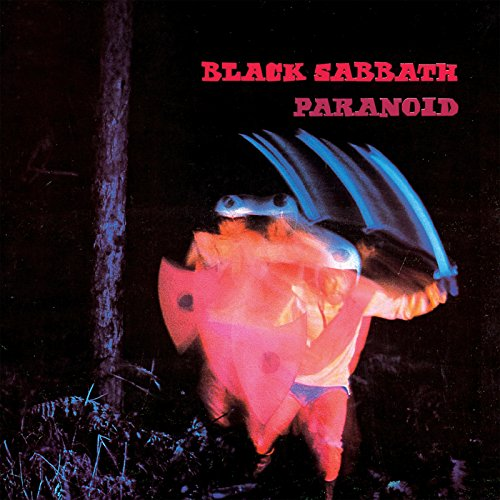
\includegraphics[width=2in]{paranoid.jpg}} about. 

\subsubsection{Prevention and Handling of Multiple Accounts}

It is important to make sure that trying to thwart the system by making multiple accounts or lying about services is either not possible or not worthwhile. Our main approach to this is making the initial trust rating for clients neutral and displaying the number of transactions attached to an account, such that making multiple accounts does not necessarily help the client in accessing services. Essentially, we make it not worthwhile for users to have multiple accounts because of our reputation propagation algorithm. 

\subsubsection{Prevention of Boosting}
Additionally, we propose a solution to the threat of \textit{boosting}, in which one person makes multiple accounts in order to fake transactions between their own accounts and increase their reputation, or multiple users collude to give each other good ratings without actually going through with a transaction. Silkworm does not keep track of transaction history beyond what is used to update the reputation score of another user. To maintain this element of the system, we propose using a hash table to anonymously keep track of the fact that a rating has been given. We also consider accounts suspicious if they have a large number of transactions but no reputation (meaning someone has been creating accounts to make transactions with each other) or accounts that are relatively disconnected when one examines the network of invitations. 

When a user rates another user at the closing of a transaction, their ID will be hashed and the corresponding bucket will be set to the change in the rating. If there is a collision between two positive ratings, the higher of the two positive ratings will be kept. Neutral ratings are never kept. If there is a collision between a positive and a negative rating, the rating with the greater magnitude (after accounting for a certain margin of difference $\epsilon$) is kept, which will ensure that a user with no reputation cannot easily undo the rating of a user with a strongly positive reputation. In all cases, accepting a new rating would also mean undoing the changes that the old rating made before recalculating the new score. If applicable, a user's reputation score will always take the reputation scores of their referrers into account, and they will be kept separately from this hashtable.

With a small hashtable and a large number of users, this method would effectively divide all users into random cohorts, allowing the ratings attached to each bucket to remain anonymous. If the hashtables and hash function are compromised, the adversary would not be able to figure out which users gave which ratings.

\subsubsection{Other System Threats}
Another attack to the system we must prevent against is a client willingly sharing their phone/account with another, potentially untrustworthy client. A client with a positive trust rating would be disincentivized from doing this because it would cause their reputation to only be as high as the least trustworthy member of the team behind the account. 

Additionally, as with many invite-only services, if a user $A$ invites another user $B$, but $B$ is found to be untrustworthy by others, then not only is $B$ punished with a negative trust rating, but $A$ is as well. This will deter users from inviting people unless they are very certain that the person is reputable.

\subsection{Known Challenges}

\subsubsection{Selling Accounts}
Because new users' ratings start so low, this could incentivize new entrants into a channel (or untrustworthy people) to buy accounts from inactive users with positive reputation scores instead of building their reputations from scratch. A possible solution would be attaching the account to the IMEI of a phone, which would raise the cost barrier for such a transaction, but we chose not to do this. Additionally, we would like for users to not have to worry about inputting sensitive personal information into the central database in case it is corrupted. We generally make the assumption here that an account with a high reputation would not sell their account because they care about their high reputation and also would not want another user to take advantage of the system. 

\subsubsection{Heuristics}
One challenge of implementation of Silkworm will be selecting values of $\rho, \mu, \tau, \beta$, and $\gamma$
such that the system functionality is tuned to a reasonable level. The manipulation of these values can be used to modify:
\begin{itemize}
    \item $\mu$, How fast a user can change reputation by performing transactions
    \item $\beta$, What range of values are considered reputable
    \item $\gamma$, How much an invited user should be relied up based on the reputation of the inviter
    \item $\rho$, How much an invitee's change in reputation should impact the inviter's.
    \item $\tau$, The trust rating scale assigned by the application.
\end{itemize}
Needless to say the assignment of these values could be the product of several comprehensive studies. As a result, we choose to acknowledge that the selection of these variables is a mathematical challenge, which we aim to learn more about in future work. 

\subsubsection{Compromise of the database}
As with all centralized systems, database compromise is a potential problem. So far, there has been no mention of which values are kept in cleartext and which are stored after one-way hashing. More analysis needs to be done to determine what an adversary can and cannot deduce from a compromised database, and proper precautions should be taken. This motivates our commitment to not storing completed transactions, as without those, an attacker cannot look through the acquired database in order to reassemble transaction-based relationships between users. Additionally, we require minimal information from users who make accounts in general, as we have our schemes for making multiple account not beneficial, such that the biggest threat in this situation would be for an attacker to steal plaintext accounts information and use a reputable account to make bad transactions. One solution to this would be implementing something similar to CryptDB's \cite{CryptDB} scheme of partially homomorphic encryption, such that we could perform calculations on encrypted information in the database. 

\subsubsection{Malicious User Channel Creation and Collusion}
There are certain indicators that may be present if a channel is maliciously controlled. One would be that all users have generally similar amounts of reputation and transaction scores, that access patterns seem relatively uniform (as opposed to timed when a group humans would use the service), or that transactions are mostly completed in very short amounts of time. Some possible protections mentioned were having related communities advertise their real Silkworm channel, such that users know which one to sign up for, or to keep track of the total number of flagged transactions within a channel and then add a flag to a channel after a certain threshold. We may also consider analyzing the invitation provenance graphs to see if the patterns make sense for a real group of users. The central authority may also step in to blacklist certain channels if they seem to having unusual patterns of use. It is also worth noting that this attack is much harder to do in in a private channel, as each user who was not invited by the creator must have increased their own reputation by some unit in order to invite others, and this would appear as a very specific type of invitation graph (all users invited by creator and no others). 

\section{Related Work}
There have been many attempts to create similarly styled reputation networks. However, most of them either involve some sort of currency that must be exchanged, keep track of transactions, or do not take into account reputation weighting or negative feedback. 

Many reputation systems have been integrated into review websites, like Yelp, which do not try to provide pseudonymity for either party. \cite{HBSPaper} describes current problems with identity-heavy rating systems. One such problem is the potential for discrimination in selecting someone to perform a transaction with. In cases where the users have images of themselves attached to their reputation profiles, other users may be biased in their selection of clients or SPs. Silkworm has an advantage in this case as long as the initial communication is free of identity markers like race or gender, there is a much smaller chance of selection bias. In cases where the transaction necessarily requires an in person meeting, this is more difficult to deal with, and we acknowledge that the reputation system may perpetuate some degree of bias within the communities. 

Other systems, like \cite{RepCoin}, often have some notion of reputation \textit{exchange}, where reputation is represented as a currency. While this idea is compelling, we prefer a model in which one does not have to give up their own reputation points in order to make a transaction with another, as this may too strongly disincentivize users from holding transactions with others. Because of our propagation algorithms for reputation based on transactions and invitations, a user is already deterred from inviting untrustworthy users. 

Another problem that is sometimes not addressed is the weighting of reputation propagation. In \cite{AnonRep}, though it has many advantages in terms of avoiding a currency representation and including negative feedback, it does not allow for relative weighting of reputation updates. This is what allows Silkworm to get rid of transaction history, as users in a non-maliciously-created channel would not be able to access enough reputation points to increase each other's reputation to any believable amount. 

\section{Conclusion and Future Work}
Silkworm improves upon many preexisting network of trust/reputation systems: it provides a reliable way of aggregating reputation ratings for users, prevents or disincentivizes malicious behavior, and is easy to use on top of preexisting communication platforms. However, some components of it require further analysis and improvement before it can be released into the wild.

\textit{Handling Multiple Accounts and Account Sharing:} We do not believe that allowing one user to own multiple accounts or multiple users to share one account will provide them any advantage. However, we would need to run an experiment to fully determine whether this is actually true, and if not, come up with other ways to disincentivize these behaviors.

\textit{Boosting Prevention:} In the hashtable method described in section 5.1.2, only the most influential person in each cohort will have a say in a user's overall reputation score, which could unfairly override the opinions of many more users. Implementing this in a way that balances input from many users may require adding more metrics to each hashtable bucket.

\textit{Heuristics and Tuning:} Section 3 introduces a few formulas and variables for calculating reputation ratings upon invitation or a new transaction. Due to the recursive nature of the reputation scores, each of these variables will need to be tuned pre-production, potentially to a channel-specific extent.

\textit{Data Protection:} The database could be compromised, so we should carefully analyze what an adversary can see in plaintext, and whether users' identities can be deduced from analyzing the database contents.

\section*{Acknowledgments}
We would like to thank Prof. James Mickens for an awesome semester of CS263!

%%%%%%%%%%%%%%%%%%%%%%%%%%%%%%%%%%%%%%%%%%%%%%
%%%%%%% old info %%%%%%%%%%%%%%%%%%%%%%%%%%%%%

%Because of the negative connotations with adult content and sex work in particular, there has been very little motivation for tech communities to focus on building or extending tools to be used by sex workers. The trope of the spam bot or script kiddie posing as a sex worker in order to steal personal information has strongly impacted how online community standards treat sex workers. For instance, Facebook does not allow one to use a fake name, partially due to the fear that a scammer will impersonate a woman and contact men in order to get personal information from them. Additionally, many marketplace or donation websites explicitly forbid adult services to be transferred on their platforms. Recently, Patreon updated its terms of service to make it against the rules to incorporate any type of sex work into one's donor rewards. These examples are problematic because they are effectively barring sex workers, who depend on their work to make a living, from using well-constructed and safe methods for their communication and transactions.

%It is also important to note that much of the initial movement of users onto the platform is dependent on the preexisting communities of sex workers both online and in person. Because sex workers are already doing so much to try to keep each other safe, the networks that exist are a great starting point for allowing workers to start using the service. This, as we will discuss later, is what makes it possible for workers to start out with higher trust ratings and also makes it possible to recognize users who attempt to sign up as sex workers despite not being one—the service would be invite-only for workers, such that those who wish to impersonate workers could not do so easily.

%The service we design can benefit both parties by allowing sex workers to see that a client has had a good history with other workers, and also allowing clients to see that a sex worker is not a bot or scam artist, while also enabling a worker and client to each maintain their anonymity.

%\section{Worker-Client Network and Anonymity}

%In order to allow sex workers to confirm with some amount of certainty that a client is not dangerous/does not have a dangerous history, they must be able to have some knowledge of that client's history with other workers. A difficult way to do this would be to allow the worker to know the client's name in order to perform a background check, which is not only mathematically hard to do without revealing the identity of the worker, but also dissuades the client from using the tool due to visibility of their identity. There is a large amount of value placed by the client in having their name not be made available to the service, such that anonymity must be preserved in the storage of user information. 

%To allow workers to have a better picture of client history while allowing the client to remain anonymous, we allow for the following:
%\begin{itemize}
 %   \item A worker to rate an interaction with a client, on a $[-1,1]$ scale, 24 hours after the interaction has taken place. 
 %   \item A worker to attest to the trustworthiness of a client without a transaction having taken place. This is to allow for existing clients to have positive trust ratings in the system without having to rely on only new interactions.
%    \item A worker to have some neighborhood of connected workers, marked by whom they were invited by and who they invited, and additional workers at their discretion, such that they can see if someone in their neighborhood has had an interaction with a client before. In this case, the identification of the client can be either through the service used to connect with them (a dating site) or the client's system ID code. 
%\end{itemize}

%In order to support some of the safety features, we require that the worker and client agree on a location and time for an in-person meeting, and just a time for an online meeting. This will make it possible to restrict the timeline for rating the trust of a client/worker. 



%\section{Transaction Storage}

%\section{Implementation and Usage}

%\subsection{Displays of Trustworthiness}

%A sex worker should be able to use the service to tell who is positively trustworthy, but will not necessarily be able to tell who is potentially dangerous. Consistent positive interactions with sex workers will allow for a client to build up a good "trust rating" such that workers can feel safer interacting with the client. On the other hand, because we cannot guarantee that a client will not make multiple accounts to try to avoid past negative ratings, the best we can do is to allow sex workers to deny services to clients who have blank or negative transaction histories. The most direct way of representing trust would be on a -1 to 1 scale, such that a user could start out in a neutral (0) state. 

 

%\subsection{Ease of Use}
%One of the most important parts of the system is its ease of use and accessibility. A difficult to figure out or clunky interface would deter clients from using it, which defeats the purpose of having trust associated with users. Many clients have difficulty even using PGP.\cite{Hexe} To account for this, an interface that we believe would make the most sense would be similar to a two-factor authentication app that would work on top of one's existing methods of contact. A worker may have a profile on an online dating website, to which they can have a reference to their 6-character alphanumeric identification code. When contact between a worker and client is initiated, the two will confirm that they are both on the service. If not, the worker may either ask the client to join or refuse contact. Assuming both are on it, the worker and client can both send a secret random number to each other's accounts in the service to confirm each has truly has control of the account they send, which will then be repeated back to them in the messaging service they are using. Because each party has control over the random number they are sending, it is extremely unlikely that it will be guessed by the other side. There is no concern for a brute-force attack to guess numbers here, because they are sent to the other party, such that there is only one "guess" to be made before it is obvious whether or not the person messaging owns the account.   

%\section{Ethical Challenges}

%The problem we are attempting to address is not to be taken lightly, as it is a question of physical safety. Because of this, in the worker interface, we include emergency contact information for other workers in the network, such that if a transaction is seen as incomplete or otherwise suspicious, action can be taken to protect the worker. To make this simpler, we do not allow the rating of a transaction to be done within 24 hours of its initiation. This means it will be more difficult for a client to force or guilt a worker into proving them a positive rating. If the rating is not confirmed by the worker withing the following period of 24 hours, a message will be sent to the emergency contact(s) which includes the ID code of the client as well as the location of the in-person meetup. 

%We must also consider the danger of the service becoming a honeypot for law enforcement agents who would be able to deduce that a person who is part of the worker side of the network is necessarily a sex worker. There is strength in numbers on platforms like dating websites, such that the mere act of being there does not imply one is a sex worker, despite the presence of sex workers on dating sites. 

% Another modification of PGP is the expansion of a trusted neighborhood through indirect trust relationships, meaning that if one user's trusted neighbors have all trusted another user not currently included in the first user's trusted neighbors, that collective feedback can be fully trusted by the user. (I don't think we used this anywhere so now it's just chilling here)

% we don't need to worry about fake ratings because each rating can only come after a valid transaction


{\footnotesize \bibliographystyle{acm}
\bibliography{sample}}


\theendnotes

\end{document}
